% !TEX TS-program = pdflatex
% !TEX encoding = UTF-8 Unicode

% This is a simple template for a LaTeX document using the "article" class.
% See "book", "report", "letter" for other types of document.

\documentclass[12pt]{article} % use larger type; default would be 10pt

\usepackage[utf8]{inputenc} % set input encoding (not needed with XeLaTeX)

%%% Examples of Article customizations
% These packages are optional, depending whether you want the features they provide.
% See the LaTeX Companion or other references for full information.

%%% PAGE DIMENSIONS
\usepackage{geometry} % to change the page dimensions
\geometry{a4paper} % or letterpaper (US) or a5paper or....
% \geometry{margin=2in} % for example, change the margins to 2 inches all round
% \geometry{landscape} % set up the page for landscape
%   read geometry.pdf for detailed page layout information

\usepackage{graphicx} % support the \includegraphics command and options

% \usepackage[parfill]{parskip} % Activate to begin paragraphs with an empty line rather than an indent

%%% PACKAGES
\usepackage{booktabs} % for much better looking tables
\usepackage{array} % for better arrays (eg matrices) in maths
\usepackage{paralist} % very flexible & customisable lists (eg. enumerate/itemize, etc.)
\usepackage{verbatim} % adds environment for commenting out blocks of text & for better verbatim
\usepackage{subfig} % make it possible to include more than one captioned figure/table in a single float
% These packages are all incorporated in the memoir class to one degree or another...

%%% HEADERS & FOOTERS
\usepackage{fancyhdr} % This should be set AFTER setting up the page geometry
\pagestyle{fancy} % options: empty , plain , fancy
\renewcommand{\headrulewidth}{0pt} % customise the layout...
\lhead{}\chead{}\rhead{}
\lfoot{}\cfoot{\thepage}\rfoot{}

%%% SECTION TITLE APPEARANCE
\usepackage{sectsty}
\usepackage{helvet}
\usepackage{titlesec}
\usepackage{inputenc}
\usepackage{amsmath}
\allsectionsfont{\sffamily\mdseries\upshape} % (See the fntguide.pdf for font help)
\titleformat{\section}
{\normalfont\fontsize{16}{19}\sffamily\bfseries}
{\thesection}
{1em}
{}

\titleformat{\subsection}
{\normalfont\fontsize{12}{17}\sffamily\bfseries}
{\thesubsection}
{1em}
{}

\titleformat{\subsubsection}
{\normalfont\fontsize{12}{17}\sffamily\bfseries}
{\thesubsubsection}
{1em}
{}
% (This matches ConTeXt defaults)

%%% ToC (table of contents) APPEARANCE
\usepackage[nottoc,notlof,notlot]{tocbibind} % Put the bibliography in the ToC
\usepackage[titles,subfigure]{tocloft} % Alter the style of the Table of Contents
\renewcommand{\cftsecfont}{\rmfamily\mdseries\upshape}
\renewcommand{\cftsecpagefont}{\rmfamily\mdseries\upshape} % No bold!

%%% END Article customizations

%%% The "real" document content comes below...

%\date{} % Activate to display a given date or no date (if empty),
         % otherwise the current date is printed 
\usepackage{url}
\usepackage{float}
\usepackage{indentfirst}

\setcounter{tocdepth}{3}

\graphicspath {{Resources/}}

%\setlength{\parindent}{4em}

\begin{document}
\input{"title_page.tex"}
\tableofcontents
\newpage
\listoffigures
\newpage
\listoftables
\newpage

\newpage
\section{Theoretical Background}
\subsection{Introduction to Deep Learning}
\vspace{1em}
Machine learning (ML) is the scientific study of algorithms and statistical models that computer systems use to effectively perform a specific task without using explicit instructions, relying on patterns and inference instead. Machine learning algorithms build a mathematical model of sample data, known as "training data", in order to make predictions or decisions without being explicitly programmed to perform the task. Machine learning algorithms are used in a wide variety of applications, such as email filtering, and computer vision, where it is infeasible to develop an algorithm of specific instructions for performing the task. The represantation of data fed into a ML algorithm plays a major role, as it affects the algorithm’s ability to efficiently extract signals and make decisions. Thus, it is important to carefully select the information included in such a representation. Formally, the representation is com- posed of multiple features extracted from raw data. The process of creating new features requires good and intuitive understanding of the data at hand, becoming incrementally time-consuming with the sophistication of the new features. Thus, the biggest challenge of handcrafted features is deciding which features are important and relevant to the problem \cite{Goodfellow-et-al-2016}\par



\section{Neural Networks}
This section introduces the main concepts related to neural networks. Neural networks have been around since the 1940s and could initially handle only one hidden layer. But with the development of technologies and hardware, it became possible to build deeper, more effective architectures, which lead to deep learning as we know it today. \par



\subsection{Brief History}


At first, neural networks were inspired by the functioning of the biological brain, which is why deep learning is also called artificial neural networks (ANNs)~\cite{Goodfellow-et-al-2016}. In biology, a neuron is the cell that receives, processes and transmits information to other neurons through connections called synapses~\cite{neuron}. On the other hand, artificial neurons are defined as computational units (usually mathematical functions) that take one or more inputs and generate an output. \par

McCulloch and Pits designed an initial version of the neuron as a linear model in 1943, aiming to replicate brain function~\cite{REF:11}:


\begin{equation}
f(x,w)=x_1*w_1 +x_2*w_2 +...+x_n*w_n
\end{equation}
where $x_1, ..., x_n$ are the input values and $w_1, ..., w_2$ is a set of hand-chosen weights.

\subsection{Components of an artificial neural network}

A simple artificial neural network (ANN) consists of an input layer, hidden layer and output layer, where the values of the hidden layer are used as inputs for the output layer. A network with several layers is known as a deep neural network. Data flows through the neurons of the layer. Each neuron transforms the input it receives and sends it to the next layer. The neurons share the same characteristics regardless of the layer they are part of. \par



The Neuron, also called a node, is the basic unit of a neural network. Its main components include inputs,
weights, activation function and output(s). From a high-level point of view, the inputs are multiplied by 
weights, then an activation function is applied to the result and finally, another function computes the output~\cite{REF:12}~\cite{REF:13}. \par


\begin{itemize}
	\item Weights are defined as adaptive coefficients, whose values are changed during the learning process. They represent the strength of the connection between units. A weight decides how much impact the input will have on the output
	
	\item The summation function helps combine the input and weights, before passing the result to the activation function. Denote the input as $X = [x_1, x_2, ...x_n]$ and the weight vector as $W = [w_1, w_2, ...w_n]$.\\
	The summation function could be defined as the dot product between these two vectors:\\
	\begin{equation}
	X \cdot W =x_1 \cdot w_1 +x_2 \cdot w_2 +...+x_n \cdot w_n
	\end{equation}

	
	The summation function could instead compute the minimum, maximum, etc. depending on the designated network architecture. The simplest form of an artificial neuron is a linear function which computes the weighted sum of inputs, to which, optionally, bias can be added:
	\begin{equation}
		y = \sum_{i=1}^{i=n}(x_i \cdot w_i) + b \textnormal{, where $b$ is the bias, $x_i \in X, w_i \in W$}
	\end{equation}

	
	\item The activation function transforms the result of the summation function (usually) in a non-linear way. Typically, it has a squashing effect. It serves as a threshold. It divides the original space into two partitions. Its main purpose is to make the neural network non-linear. We denote the activation function as $g$
	\begin{equation}
		y = g(\sum_{i=1}^{i=n}(x_i \cdot w_i) + b) \textnormal{, where $b$ is the bias, $x_i \in X, w_i \in W$}
	\end{equation}

	
	\begin{figure}[h]
		\caption[Common activation functions]{Common activation functions~\cite{activation_fig} }
		\centering
		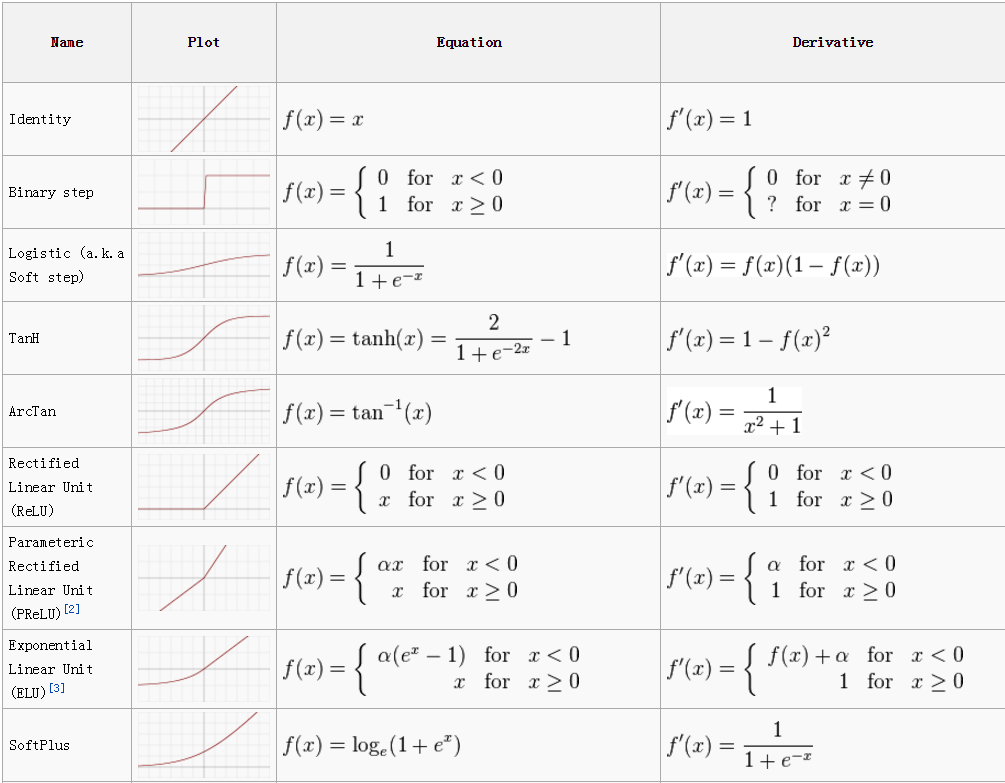
\includegraphics[width=1\textwidth, height=\textheight, keepaspectratio]{activation}
	\end{figure}
	\item The output is usually the result of an activation function
	
\end{itemize}

\clearpage
\subsection{Under-fitting and Over-fitting}
%reformulat + surse noi

Neural networks are able to learn complicated non-linear functions to fit any training set. On the downside, this may lead to over-fitting where the neural network learns the training data so well that it is unable to generalize on new, unseen data. This problem can especially occur on datasets with a small amount of data to learn from. \par

Under-fitting, the counterpart of over-fitting, happens when a machine learning model isn’t complex enough to accurately capture relationships between a dataset’s features and a target variable. Under-fitted models result in problematic outcomes on new data or data that they  were not trained on, and many times perform poorly even on training data. \par


\begin{figure}[h]
	\caption[Example of over-fitting and under-fitting]{Example of over-fitting and under-fitting~\cite{vitaflux}}
	\centering
	\includegraphics[width=1\textwidth, height=\textheight, keepaspectratio]{"resources/overfitting"}
\end{figure}

\subsection{Convolutional Neural Networks}
\par
Convolutional Neural Networks (CNNs) are a class of Deep Neural Networks,
specialized in analyzing images. Their development was inspired by biological processes.
The connectivity pattern between neurons resembles the animal visual cortex~\cite{cnn}. \par

\begin{figure}[h]
	\centering
	\caption[Typical convolutional neural network architecture]{Typical CNN architecture~\cite{cnn_fig}}
	\label{fig:cnn}
	\includegraphics[width=1.1\textwidth, height=1.5\textheight, keepaspectratio]{"resources/typical_cnn"}
\end{figure}

\par
A convolutional neural network consists of an input and an output layer, as well as multiple hidden layers. The hidden layers are typically convolutional layers, RELU layers, pooling layers, fully connected layers and normalization layers~\cite{cnn_git}.

\begin{itemize}
	\item \textbf{Convolutional} layers are the core building block of convolutional networks. They are responsible for feature extraction and do most of the computation
	\item \textbf{Pooling} layers reduce the dimension of the data by combining the outputs of neuron clusters at one layer into a single neuron in the next layer
	\item \textbf{Normalization} layers apply a transformation that maintains the mean activation close to 0 and the activation standard deviation close to 1
	\item \textbf{Fully connected} layers link every neuron in one layer to every neuron in another layer
	\item \textbf{Dropout} layers have a \% chance to deactivate the neurons of a particular layer. This is a technique used to improve over-fitting by improving generalization. Forcing neurons to deactivate forces the network to learn the same "concept" with different neurons. It is mostly used after fully connected or pooling layers
\end{itemize}




\newpage
\subsection{Convolutional Neural Networks}
\par
Convolutional Neural Networks (CNNs) are a class of Deep Neural Networks,
specialized in analyzing images. They were inspired by biological processes.
The connectivity pattern between neurons resembles the animal visual cortex.
\cite{cnn} \par

\subsubsection{Find subsections}


\newpage



\newpage
\subsection{Music Transcription}
In music, transcription is the process of creating a music sheet from a piece or sound. The sheet contains music notation, which consists of different symbols that can be interpreted by musicians, hence it is important for various reasons. Without it composers such as Mozart and Beethoven couldn't have passed their masterpieces across generations. In modern days it helps musicians play songs they never heard before. It's also universal so even if two musicians don't speak the same language, they can read the same notation.

\subsubsection{Traditional Music Transcription}
In the beginning transcription was done by humans. It's also called musical dictation in ear training pedagogy. \cite{human_transcription} It is a skill by which musicians learn to identify pitches, intervals, melody, chords and other elements of music solely by hearing. It is a really hard skill, requires serious training and study and even the best don't have 100\% accuracy. \par

There are some tools to help with the process:
\begin{itemize}
	\item Musical instruments, help musicians test for certain sounds, trying to mimic what they hear
	\item Tape recorders
	\item Nowadays software
\end{itemize}

\subsubsection{Automated Music Transcription}
The term "Automated Music Transcription" was used for the first time in 1977, by audio researchers James A. Moorer, Martin Piszczalski, and Bernard Galler \cite{transcription}. With their knowledge about digital engineering they believed that computers could be programmed to analyze digital recordings of songs such that they could identify things like rhythm, melodies, pitch, bass lines. It's not an easy task. For more than three decades researchers have been trying to crack it open. \par

Fundamentally, AMT is about identifying the pitch and duration of played notes, so they can be converted in traditional music notation on a sheet. \par

It has many advantages over traditional transcription:
\begin{itemize}
	\item Aids experienced musicians in the process of transcribing pieces, increasing their accuracy.
	\item Makes music transcription available to more people, especially beginners, giving them a chance to share their ideas with others.
	\item Helps people learn new songs. There are a lot of music sheets online that are not free. 
	\item It speeds up the process. Manual transcription takes a lot of time.
\end{itemize}

\newpage
\section{Related Work}

Automatic music transcription (AMT) has been attempted since the 1970s and polyphonic music transcription dates to the 1990s \cite{REF:1}
\par

\subsection{State of the art in AMT}

There has been substantial progress made in the field of AMT. Neural networks, in particular, have met and surpassed the performance of traditional pitch recognition techniques on polyphonic audio.
\par

A model used in \cite{REF:2} uses 87 Support Vector Machine (SVM) classifiers to perform frame-level classification with the advantage of simplicity, and then a Hidden Markov Model (HMM) post-processing was adopted to smooth the results. On top of it, Deep Belief Network(DBN) was added to learn higher layer representation of features in \cite{REF:3}. Since none of the approaches has reached the same level of accuracy as human experts, most music transcription work is completed by musicians. With the development of deep learning in recent years, many researchers were inspired to apply networks to accomplish AMT. A model based on Convolutional Neural Networks (CNN) was proposed in \cite{REF:4}. More models adopted Reccurent Neural Networks (RNN) or Long Short-Term Memory (LSTM) due to its capability of dealing with sequential data \cite{REF:1} \cite{REF:5} \cite{REF:6}. In \cite{REF:7}, 5 models were compared and the ConvNet model was reported as resulting in the best performance.
\par

The first majort AMT work is Smaragdis et al.\cite{REF:8}. This approach uses Non-Negative Matrix Factorization (NMF). This is the main methodology employed in software for automatic transcription, but it has it's limitations. For example, it needs to know how many individual notes are desired for the transcription (information that is not always available).
\par

The next work worth mentioning is Emiya et al.\cite{REF:9}, not because of their transcription system (as it was out-performed in the same year), but because of the dataset they created that has become the standard in evaluating any multi-pitch estimation system. They created the MIDI-Aligned Piano Sounds (MAPS) data set composed of around 10,000 piano sounds either recorded by using an upright Disklavier piano or generated by several virtual piano software products based on sampled sounds. The dataset
consists of audio and corresponding annotations for isolated sounds, chords, and complete pieces of piano music.
\par

Sigtia et al.\cite{REF:10} built the first AMT system using CNN, outperforming the state of the art approaches using NMF. Convolutional
Neural Networks are a discriminative approach to AMT, which has been found to be a
viable alternative to spectrogram factorization techniques. Discriminative approaches
aim to directly classify features extracted from frames of audio to the output pitches.
This approach uses complex classifiers that are trained using large amounts of training
data to capture the variability in the inputs, instead of constructing an instrument
specific model. 
\par

Sigtia et al. \cite{REF:10} explored various models for pitch detection. In addition to CNNs, they tried Deep Neural Networks and Recurrent Neural Networks. The results have shown that their CNN based model outperformed the others for this task. In their paper, they propose a Music Language Model (MLM) that's based on RNNs in order to handle the polyphonic musical data. \cite{benetos}
\par

There are some products on the market, AnthemScore for example, that use CNNs for AMT. They approach note detection as an image recognition problem by creating spectrograms of the audio. They show how the spectrum or frequency content changes over time. The method used for creating the spectrograms is the constant Q transform instead of the more common Short Time Fourier Transform (STFT) method.
\par

Melodyne is a popular plugin used for Music Transcription and Pitch Correction. It costs up to \$700. 	
The Melodic and Polyphonic algorithms offer you, in the case of vocals as well as both mono- and polyphonic instruments, full access to the notes of which the sound is composed as well as to their musical parameters.
There's no public information about what approach they used.
\par

\subsection{CNN approach to AMT}




\newpage
	\bibliography{references}
	\bibliographystyle{ieeetr}

\end{document}
